The number of active authors in Git is shown below, giving us a quick look of contributors evolution as compared to previous ones.

\begin{tabular}{p{9cm} p{5cm}}
	\vspace{0pt} 
	\hspace*{-6cm}  
	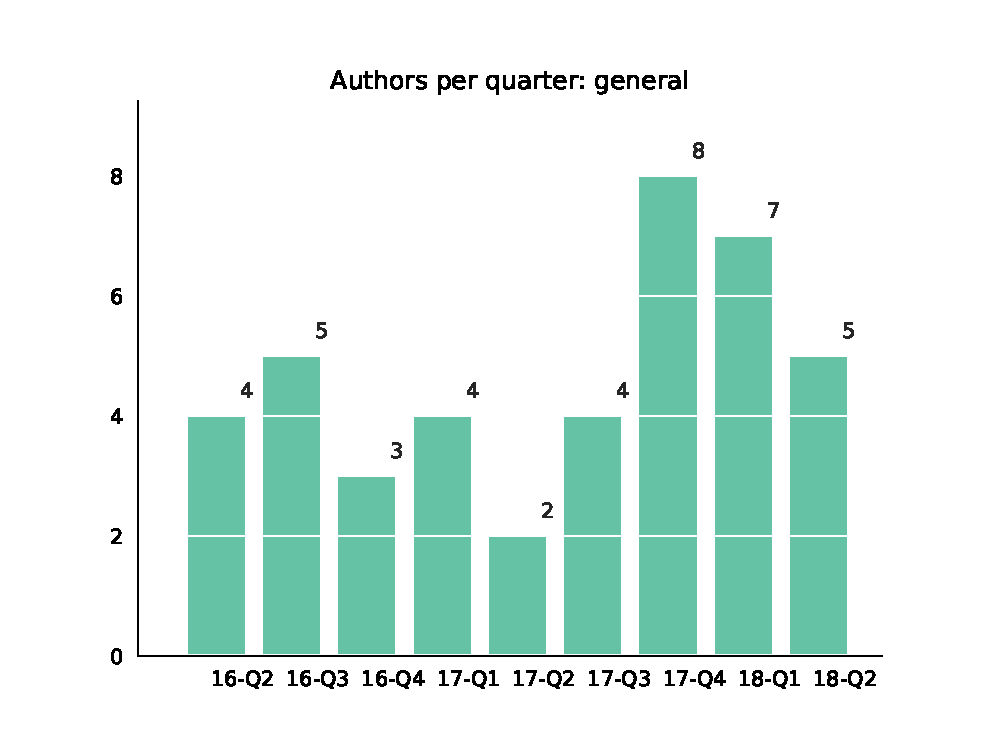
\includegraphics[scale=.75]{community/git_authors.eps}
	& 
	\vspace{0pt}
	\begin{tabular}{l|l}%
		% specify table head
		\bfseries Period & \bfseries Active Authors 
		% use head of csv as column names
		\csvreader[head to column names]{community/git_authors.csv}{}
		{\\\Date & \authors}
	\end{tabular}
\end{tabular}

In addition, the table below offers a quick glance of the most active authors in Git in the whole period of time shown in the bar chart above. 

\begin{tabular}{p{7cm} p{5cm}}
	\vspace{0pt}
	\begin{tabular}{l|l}%
		 % specify table head
		\bfseries Author & \bfseries Commit (s)
		% use head of csv as column names
		\csvreader[head to column names]{community/git_top_authors.csv}{}
		% specify your coloumns here
		{\\\hline\csvcoli&\csvcolii}
	\end{tabular}
\end{tabular}
\\
\\
In a similar way, the table below shows the same information grouped by organization instead of author.

\begin{tabular}{p{7cm} p{5cm}}
	\vspace{0pt}
	\begin{tabular}{l|l}%
		% specify table head
		\bfseries Organization & \bfseries Commit (s) 
		% use head of csv as column names
		\csvreader[head to column
		 names]{community/git_top_organizations.csv}{}
		 % specify your coloumns here
		{\\\hline\csvcoli&\csvcolii}
	\end{tabular}
	\end {tabular}
\\
\\